\documentclass{article}
\author{Isaac B Goss}
\title{Compilers Assignment 3}
\date{Wednesday, December 6, 2017}

\usepackage{amsmath}
\usepackage{amsthm}
\usepackage{enumitem}
\usepackage[margin=0.8in]{geometry}
\usepackage{graphicx}

% ============ USED FOR OUR FORMAT ============
\newtheorem{thm}{Claim}
\providecommand{\prob}[1]{\section*{Problem #1}}
\providecommand{\soln}{\textbf{Solution: }}
\providecommand{\image}[1]{
    \begin{center}
        \includegraphics[width=0.5\textwidth]
            {#1}
    \end{center}
}
\providecommand{\tightlist}{
    \setlength{\itemsep}{0pt}\setlength{\parskip}{0pt}
}

% ============ USED FOR CODE LISTINGS ============
\usepackage{listings}
\usepackage[usenames,dvipsnames,svgnames]{xcolor}
\definecolor{javagreen}{rgb}{0.25,0.5,0.35}
\lstset{
    basicstyle   = \footnotesize,
    commentstyle = \color{javagreen},
    frame        = single,
    language     = C,
    stringstyle  = \color{orange},
    numbers      = left,
    showstringspaces=false,
    deletekeywords = {len, max, format, min},
    morekeywords = {yield, function, then, do, to},
    keywordstyle = \color{blue},
    escapeinside = {(*} {*)}
}


\begin{document}
\maketitle

\prob{1}
\begin{center}
    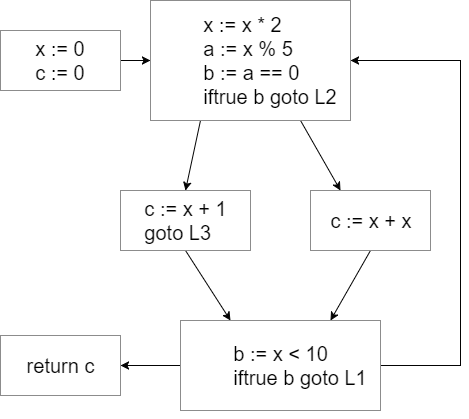
\includegraphics[width=0.5\textwidth]{ControlFlowGraph}
\end{center}

\prob{2}
\begin{center}
    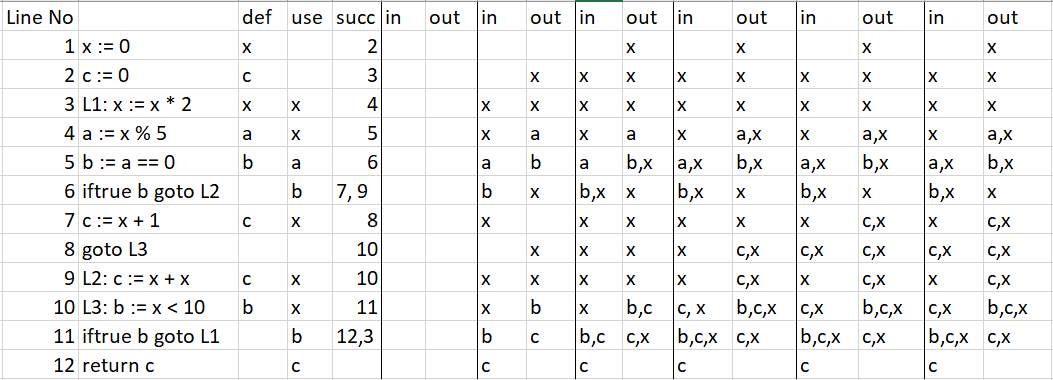
\includegraphics[width=0.95\textwidth]{LivenessPic}
\end{center}


\prob{3}
\begin{center}
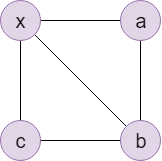
\includegraphics[width=0.2\textwidth]{InterferenceGraph}

    \begin{tabular}{l|l}
        \textbf{Name} & \textbf{Register}\\
        \hline
        x & 1 \\
        a & 3 \\
        b & 2 \\
        c & 3 \\
    \end{tabular}
    
\end{center}
\end{document}
